%\documentclass[12pt]{scrbook}
%
%\usepackage{tikz}
%\usepackage{minted}
%\usetikzlibrary{decorations.pathreplacing}
%
%\usepackage{fullpage}
%\usepackage{subfigure}
%\begin{document}
%
%
%Lorem Ipsum is simply dummy text of the printing and typesetting industry. Lorem Ipsum has been the industry's standard dummy text ever since the 1500s, when an unknown printer took a galley of type and scrambled it to make a type specimen book. It has survived not only five centuries, but also the leap into electronic typesetting, remaining essentially unchanged. It was popularised in the 1960s with the release of Letraset sheets containing Lorem Ipsum passages, and more recently with desktop publishing software like Aldus PageMaker including versions of Lorem Ipsum.
%
%
\begin{figure}
\centering

\subfigure[After the first two lines memory has been dedicated for the 
variable \mintinline{c}{a} and the pointer variable \mintinline{c}{ptrA} and
their values have been initialized.]{

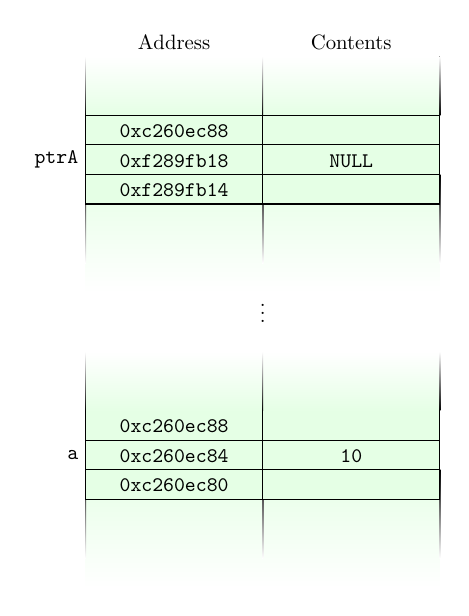
\begin{tikzpicture}[auto,scale=.75,transform shape,every node/.style={text centered}]


\path [top color=green!10!white, bottom color=white] (0,3) rectangle (6,5);
\fill [top color=black, bottom color=white] (-0.0075,3.5) rectangle (.01,5);
\fill [top color=black, bottom color=white] (2.9925,3.5) rectangle (3.01,5);
\fill [top color=black, bottom color=white] (5.9925,3.5) rectangle (6.01,5);

\draw[fill=green!10!white] (0, 4.5) rectangle (3, 5);
\node [above] (aa1) at (1.5,4.5) {\texttt{0xc260ec80}};
\draw[fill=green!10!white] (3, 4.5) rectangle (6, 5);
\node [above] (aa2) at (4.5,4.5) {~};

\draw[fill=green!10!white] (0, 5) rectangle (3, 5.5);
\node [above] (bb1) at (1.5,5) {\texttt{0xc260ec84}};
\draw[fill=green!10!white] (3, 5) rectangle (6, 5.5);
\node [above] (bb2) at (4.5,5) {\texttt{10}};
\node [left] (XX) at (0,5.25) {\texttt{a}};

\draw[fill=green!10!white] (0, 5.5) rectangle (3, 6);
\node [above] (cc1) at (1.5,5.5) {\texttt{0xc260ec88}};
\draw[fill=green!10!white] (3, 5.5) rectangle (6, 6);
\node [above] (cc2) at (4.5,5.5) {~};

%\draw [decorate,decoration={brace,amplitude=5pt},xshift=-4pt,yshift=0pt] (0, 4.5) -- (0, 6) node [text width=3cm,align=center,black,midway,xshift=-.25cm]  {\mintinline{c}{sum()} stack frame};

\path [top color=white, bottom color=green!10!white] (0,6.01) rectangle (6,7);
\fill [top color=white, bottom color=black] (-0.00725,6) rectangle (.0075,7);
\fill [top color=white, bottom color=black] (5.9925,6) rectangle (6.0075,7);
\fill [top color=white, bottom color=black] (2.9925,6) rectangle (3.0075,7);

%%%bottom

\path [top color=green!10!white, bottom color=white] (0,8) rectangle (6,10);
\fill [top color=black, bottom color=white] (-0.0075,8.5) rectangle (.01,10);
\fill [top color=black, bottom color=white] (2.9925,8.5) rectangle (3.01,10);
\fill [top color=black, bottom color=white] (5.9925,8.5) rectangle (6.01,10);

\draw[fill=green!10!white] (0, 9.5) rectangle (3, 10);
\node [above] (aa1) at (1.5,9.5) {\texttt{0xf289fb14}};
\draw[fill=green!10!white] (3, 9.5) rectangle (6, 10);
\node [above] (aa2) at (4.5,9.5) {~};

\draw[fill=green!10!white] (0, 10) rectangle (3, 10.5);
\node [above] (bb1) at (1.5,10) {\texttt{0xf289fb18}};
\node [left] (bb1) at (0,10.25) {\texttt{ptrA}};
\draw[fill=green!10!white] (3, 10) rectangle (6, 10.5);
\node [above] (bb2) at (4.5,10) {\texttt{NULL}};

\draw[fill=green!10!white] (0, 10.5) rectangle (3, 11);
\node [above] (cc1) at (1.5,10.5) {\texttt{0xc260ec88}};
\draw[fill=green!10!white] (3, 10.5) rectangle (6, 11);
\node [above] (cc2) at (4.5,10.5) {~};

%\draw [decorate,decoration={brace,amplitude=5pt},xshift=-4pt,yshift=0pt] (0, 4.5) -- (0, 6) node [text width=3cm,align=center,black,midway,xshift=-.25cm]  {\mintinline{c}{sum()} stack frame};

\path [top color=white, bottom color=green!10!white] (0,11.01) rectangle (6,12);
\fill [top color=white, bottom color=black] (-0.00725,11) rectangle (.0075,12);
\fill [top color=white, bottom color=black] (5.9925,11) rectangle (6.0075,12);
\fill [top color=white, bottom color=black] (2.9925,11) rectangle (3.0075,12);

\node (dots) at (3, 7.75) {$\vdots$};

\node[above] (x1) at (1.5,12) {Address};
\node[above] (x2) at (4.5,12) {Contents};

%\draw[fill=black] (5.75, 10.25) circle (1pt);
%\draw[blue,->] (5.75, 10.25) -- (6.5, 10.25) -- (6.5,8) -- (-1,8) -- (-1,5.25) -- (XX.west);

\end{tikzpicture}
}~~~~~~~~\subfigure[Making \mintinline{c}{ptrA} point to the variable \mintinline{c}{a}'s
memory location.  The value stored in the variable \mintinline{c}{ptrA} is a
memory address.]{

\begin{tikzpicture}[auto,scale=.75,transform shape,every node/.style={text centered}]


\path [top color=green!10!white, bottom color=white] (0,3) rectangle (6,5);
\fill [top color=black, bottom color=white] (-0.0075,3.5) rectangle (.01,5);
\fill [top color=black, bottom color=white] (2.9925,3.5) rectangle (3.01,5);
\fill [top color=black, bottom color=white] (5.9925,3.5) rectangle (6.01,5);

\draw[fill=green!10!white] (0, 4.5) rectangle (3, 5);
\node [above] (aa1) at (1.5,4.5) {\texttt{0xc260ec80}};
\draw[fill=green!10!white] (3, 4.5) rectangle (6, 5);
\node [above] (aa2) at (4.5,4.5) {~};

\draw[fill=green!10!white] (0, 5) rectangle (3, 5.5);
\node [above] (bb1) at (1.5,5) {\texttt{0xc260ec84}};
\draw[fill=green!10!white] (3, 5) rectangle (6, 5.5);
\node [above] (bb2) at (4.5,5) {\texttt{10}};
\node [left] (XX) at (0,5.25) {\texttt{a}};

\draw[fill=green!10!white] (0, 5.5) rectangle (3, 6);
\node [above] (cc1) at (1.5,5.5) {\texttt{0xc260ec88}};
\draw[fill=green!10!white] (3, 5.5) rectangle (6, 6);
\node [above] (cc2) at (4.5,5.5) {~};

%\draw [decorate,decoration={brace,amplitude=5pt},xshift=-4pt,yshift=0pt] (0, 4.5) -- (0, 6) node [text width=3cm,align=center,black,midway,xshift=-.25cm]  {\mintinline{c}{sum()} stack frame};

\path [top color=white, bottom color=green!10!white] (0,6.01) rectangle (6,7);
\fill [top color=white, bottom color=black] (-0.00725,6) rectangle (.0075,7);
\fill [top color=white, bottom color=black] (5.9925,6) rectangle (6.0075,7);
\fill [top color=white, bottom color=black] (2.9925,6) rectangle (3.0075,7);

%%%bottom

\path [top color=green!10!white, bottom color=white] (0,8) rectangle (6,10);
\fill [top color=black, bottom color=white] (-0.0075,8.5) rectangle (.01,10);
\fill [top color=black, bottom color=white] (2.9925,8.5) rectangle (3.01,10);
\fill [top color=black, bottom color=white] (5.9925,8.5) rectangle (6.01,10);

\draw[fill=green!10!white] (0, 9.5) rectangle (3, 10);
\node [above] (aa1) at (1.5,9.5) {\texttt{0xf289fb14}};
\draw[fill=green!10!white] (3, 9.5) rectangle (6, 10);
\node [above] (aa2) at (4.5,9.5) {~};

\draw[fill=green!10!white] (0, 10) rectangle (3, 10.5);
\node [above] (bb1) at (1.5,10) {\texttt{0xf289fb18}};
\node [left] (bb1) at (0,10.25) {\texttt{ptrA}};
\draw[fill=green!10!white] (3, 10) rectangle (6, 10.5);
\node [above] (bb2) at (4.5,10) {\texttt{0xc260ec84}};

\draw[fill=green!10!white] (0, 10.5) rectangle (3, 11);
\node [above] (cc1) at (1.5,10.5) {\texttt{0xc260ec88}};
\draw[fill=green!10!white] (3, 10.5) rectangle (6, 11);
\node [above] (cc2) at (4.5,10.5) {~};

%\draw [decorate,decoration={brace,amplitude=5pt},xshift=-4pt,yshift=0pt] (0, 4.5) -- (0, 6) node [text width=3cm,align=center,black,midway,xshift=-.25cm]  {\mintinline{c}{sum()} stack frame};

\path [top color=white, bottom color=green!10!white] (0,11.01) rectangle (6,12);
\fill [top color=white, bottom color=black] (-0.00725,11) rectangle (.0075,12);
\fill [top color=white, bottom color=black] (5.9925,11) rectangle (6.0075,12);
\fill [top color=white, bottom color=black] (2.9925,11) rectangle (3.0075,12);

\node (dots) at (3, 7.75) {$\vdots$};

\node[above] (x1) at (1.5,12) {Address};
\node[above] (x2) at (4.5,12) {Contents};

\draw[fill=black] (5.75, 10.25) circle (1pt);
\draw[blue,->] (5.75, 10.25) -- (6.5, 10.25) -- (6.5,8) node[below] {\mintinline{c}{ptrA = &a;}} -- (-1,8) -- (-1,5.25) -- (XX.west);

\end{tikzpicture}
}

\subfigure[Dereferencing \mintinline{c}{ptrA} and assigning a value changes
the value stored at what it \emph{points} to.]{

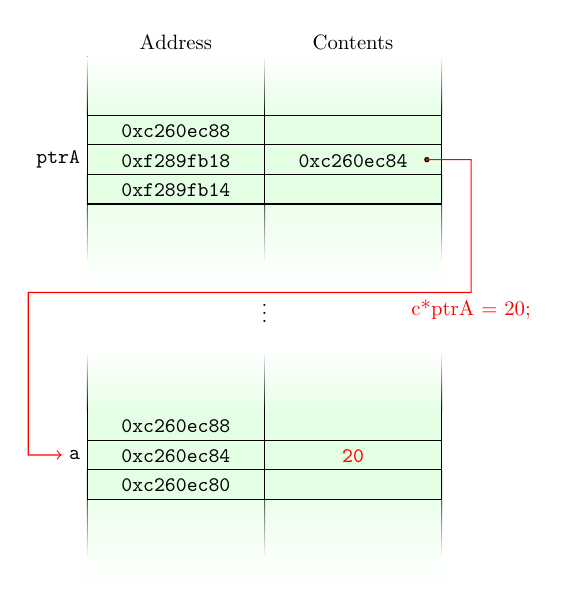
\begin{tikzpicture}[auto,scale=.75,transform shape,every node/.style={text centered}]


\path [top color=green!10!white, bottom color=white] (0,3) rectangle (6,5);
\fill [top color=black, bottom color=white] (-0.0075,3.5) rectangle (.01,5);
\fill [top color=black, bottom color=white] (2.9925,3.5) rectangle (3.01,5);
\fill [top color=black, bottom color=white] (5.9925,3.5) rectangle (6.01,5);

\draw[fill=green!10!white] (0, 4.5) rectangle (3, 5);
\node [above] (aa1) at (1.5,4.5) {\texttt{0xc260ec80}};
\draw[fill=green!10!white] (3, 4.5) rectangle (6, 5);
\node [above] (aa2) at (4.5,4.5) {~};

\draw[fill=green!10!white] (0, 5) rectangle (3, 5.5);
\node [above] (bb1) at (1.5,5) {\texttt{0xc260ec84}};
\draw[fill=green!10!white] (3, 5) rectangle (6, 5.5);
\node [above] (bb2) at (4.5,5) {\color{red}{\texttt{20}}};
\node [left] (XX) at (0,5.25) {\texttt{a}};

\draw[fill=green!10!white] (0, 5.5) rectangle (3, 6);
\node [above] (cc1) at (1.5,5.5) {\texttt{0xc260ec88}};
\draw[fill=green!10!white] (3, 5.5) rectangle (6, 6);
\node [above] (cc2) at (4.5,5.5) {~};

%\draw [decorate,decoration={brace,amplitude=5pt},xshift=-4pt,yshift=0pt] (0, 4.5) -- (0, 6) node [text width=3cm,align=center,black,midway,xshift=-.25cm]  {\mintinline{c}{sum()} stack frame};

\path [top color=white, bottom color=green!10!white] (0,6.01) rectangle (6,7);
\fill [top color=white, bottom color=black] (-0.00725,6) rectangle (.0075,7);
\fill [top color=white, bottom color=black] (5.9925,6) rectangle (6.0075,7);
\fill [top color=white, bottom color=black] (2.9925,6) rectangle (3.0075,7);

%%%bottom

\path [top color=green!10!white, bottom color=white] (0,8) rectangle (6,10);
\fill [top color=black, bottom color=white] (-0.0075,8.5) rectangle (.01,10);
\fill [top color=black, bottom color=white] (2.9925,8.5) rectangle (3.01,10);
\fill [top color=black, bottom color=white] (5.9925,8.5) rectangle (6.01,10);

\draw[fill=green!10!white] (0, 9.5) rectangle (3, 10);
\node [above] (aa1) at (1.5,9.5) {\texttt{0xf289fb14}};
\draw[fill=green!10!white] (3, 9.5) rectangle (6, 10);
\node [above] (aa2) at (4.5,9.5) {~};

\draw[fill=green!10!white] (0, 10) rectangle (3, 10.5);
\node [above] (bb1) at (1.5,10) {\texttt{0xf289fb18}};
\node [left] (bb1) at (0,10.25) {\texttt{ptrA}};
\draw[fill=green!10!white] (3, 10) rectangle (6, 10.5);
\node [above] (bb2) at (4.5,10) {\texttt{0xc260ec84}};

\draw[fill=green!10!white] (0, 10.5) rectangle (3, 11);
\node [above] (cc1) at (1.5,10.5) {\texttt{0xc260ec88}};
\draw[fill=green!10!white] (3, 10.5) rectangle (6, 11);
\node [above] (cc2) at (4.5,10.5) {~};

%\draw [decorate,decoration={brace,amplitude=5pt},xshift=-4pt,yshift=0pt] (0, 4.5) -- (0, 6) node [text width=3cm,align=center,black,midway,xshift=-.25cm]  {\mintinline{c}{sum()} stack frame};

\path [top color=white, bottom color=green!10!white] (0,11.01) rectangle (6,12);
\fill [top color=white, bottom color=black] (-0.00725,11) rectangle (.0075,12);
\fill [top color=white, bottom color=black] (5.9925,11) rectangle (6.0075,12);
\fill [top color=white, bottom color=black] (2.9925,11) rectangle (3.0075,12);

\node (dots) at (3, 7.75) {$\vdots$};

\node[above] (x1) at (1.5,12) {Address};
\node[above] (x2) at (4.5,12) {Contents};

\draw[fill=red] (5.75, 10.25) circle (1pt);
\draw[red,->] (5.75, 10.25) -- (6.5, 10.25) -- (6.5,8) node[below] {\mintinline{c}{*ptrA = 20;}} -- (-1,8) -- (-1,5.25) -- (XX.west);

\end{tikzpicture}
}


\caption[Pointer Operations]{Pointer Operations.  Pointers can be made to point to
other variable's memory locations.  You can manipulate/access values of variables 
via their pointers using dereferencing.}
\label{figure:cPointers}

\end{figure}




%\end{document}
